% !TeX root = RJwrapper.tex
\title{Functional expression study of igf2 antisense transcript in
mouse}
\author{by Marcel Kempenaar and Author Two}

\maketitle

\abstract{%
A short summary (max. 150 words) describing the original article, their
results, your research, your results and end with a short discussion.
}

\hypertarget{introduction}{%
\subsection{Introduction}\label{introduction}}

In the introduction you will focus on two things; \emph{(i)} the
research subject from the original experiment. Take the article's
abstract as inspiration but keep in mind that the target audience are
your fellow students, the biology must be made understandable. In the
next \emph{(ii)} part you can explain your planned analysis; what is
your research question, what steps are needed and if so, how will your
analysis be different from the one in the original article?

Introductory section which may include references in parentheses
\citep{R}, or cite a reference such as \citet{R} in the text, see the
last section in this document for a how-to on references.

\hypertarget{materials-and-methods}{%
\subsection{Materials and Methods}\label{materials-and-methods}}

Most likely this will be the largest section in your report (depending
on the number of images you show in the \texttt{Results} section). Take
a look at your experiments article to see how they organised its content
to see if this is also suitable for your report.

This section must at the very least contain information about the
\textbf{data}; how many samples from what organism + strain (if
applicable), what kind of data is there available (not only saying
\textbf{FPKM} but also the sequencer type that generated this data).
Also, information about all the \textbf{software} that you used during
your analysis (i.e.~\texttt{R} and its libraries, \texttt{bioConductor},
\texttt{DESeq2}, etc.) and all \textbf{methods} that you applied (both
filtering steps and statistical analysis steps). Try to use the proper
terms and symbols if needed, i.e.~``\emph{We filtered for DEGs with an}
\(\alpha\) \textless{} 0.05''.
\href{https://www.artofproblemsolving.com/wiki/index.php/LaTeX:Symbols}{Symbols}
need to be surrounded with \texttt{\$} signs, otherwise you will get an
error when knitting.

Do not show any results in this section, for instance when stating that
you filtered t-test p-values on a certain value, you do not list how
many genes were left, that is for the next section.

\hypertarget{results}{%
\subsection{Results}\label{results}}

Here you will only focus on your own results, start at the beginning but
only show the interesting results. This section works best if you
alternate between text introducing some result, a figure or table
showing the result, and a short text segment analyzing the presented
result \emph{and} introducing the next figure, etc.

Although we have worked in \texttt{R} a lot, the results are almost
never pieces of \texttt{R} code. If you have written your own algorithm
or analysis method try to present it in a formula \emph{followed} by the
\texttt{R} implementation, otherwise this section should mainly contain
figures and tables.

There are multiple methods of including a figure in this section. Figure
\ref{figure:sample_heatmap} shows the \LaTeX method (see the source
code) giving very fine control over size and placement of a figure. The
size of a figure is determined by the width of the text column, Figure
\ref{figure:sample_heatmap} is scaled as 85\% of the text width. The
\href{https://en.wikibooks.org/wiki/LaTeX/Floats,_Figures_and_Captions\#Figures}{Wikibooks.org}
website shows some examples for placement (for instance, what the
\texttt{{[}htbp{]}} means), scaling and captions.

\begin{figure}[htbp]
  \centering
  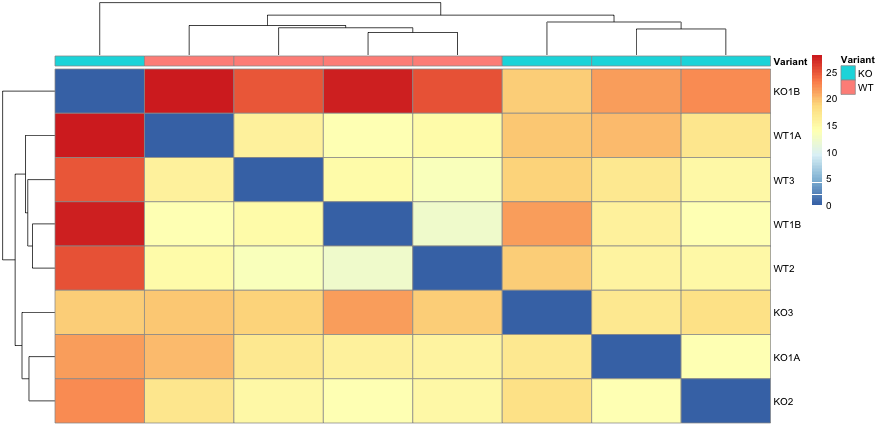
\includegraphics[width=0.85\textwidth]{images/pheatmap.png}
  \caption{Heatmap showing sample distances and clustering.}
  \label{figure:sample_heatmap}
\end{figure}

\newpage

Alternatively the previously shown \texttt{R} method using the
\texttt{PNG} library can be used which allows changing the \emph{heigth}
and \emph{width} of an image but lacks the possibility of referencing
the figure in the text, aligning the figure (the heatmap is centered),
providing a figure caption and automatic numbering of figures.

\begin{Schunk}
\begin{Sinput}
library(png)
library(grid)
img <- readPNG("images/mds.png")
grid.raster(img)
\end{Sinput}

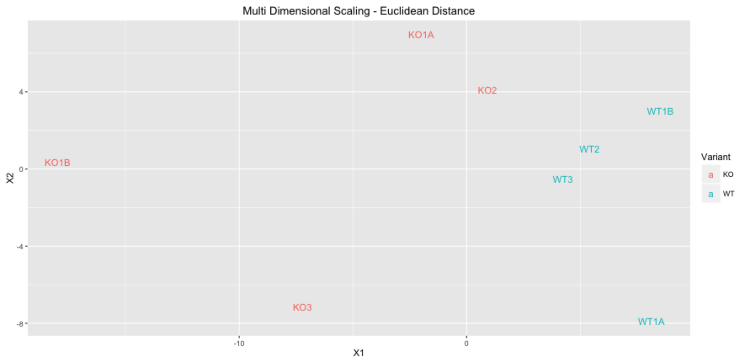
\includegraphics{report-template_files/figure-latex/MDS-Figure-1} \end{Schunk}

\hypertarget{conclusion}{%
\subsection{Conclusion}\label{conclusion}}

Limit to your \emph{own} conclusions, based on what is shown in the
\textbf{Results} section. Do not include any comparison to the original
article as that is the content of the next section, the
\textbf{Discussion}. Usually you refer back to all steps outlined in the
results section since you included it there for a reason.

\hypertarget{discussion}{%
\subsection{Discussion}\label{discussion}}

An important section in your report; here you can compare your findings
with the findings presented in the original article. If you found
exactly the same results - and that was your goal from the start - this
will be a bit shorter section and you should focus on other parts of
your research that hasn't been discussed or shown in the article,
i.e.~any findings from the exploratory data analysis or differences in
DEGs using the manual- and library-method.

Besides comparing the two `experiments', this is also the place to
discuss how reliable your results are. Did anything go wrong or did you
get unexpected outcomes using some method and if so, what did you do to
solve it or are there still open discussion points on this subject.

\hypertarget{notes-on-the-bibliography-section}{%
\subsection{\texorpdfstring{Notes on the \texttt{bibliography}
section}{Notes on the bibliography section}}\label{notes-on-the-bibliography-section}}

The last section in the report contains all the used references that are
used throughout the text in a section called the \texttt{Bibliography}.
In the text you can link to references using the \LaTeX commands (see
the source of this file for instructions). These references must be
present in a file named \texttt{RJreferences.bib} which is automatically
generated once you click the \texttt{Knit} button for the first time in
a folder with the same name as the current markdown file
(\texttt{./report-template/RJreferences.bib} for this example file).

This file containing the references can be edited in RStudio too, browse
to the folder (after Knitting) and click on the \texttt{.bib} file to
edit. If, for example, I want to add the article that is available for
the experiment used in the week 4 - 7 assignment document, I would first
lookup the paper in
\href{http://www.ncbi.nlm.nih.gov/pmc/articles/PMC3914337/}{PubMed} to
get the details and add these details to the \texttt{.bib} file as
follows:

\begin{verbatim}
@article{garcia,
    author = {Duart-Garcia, Braunschweig},
    title = {Functional expression study of igf2 antisense transcript in mouse},
    journal = {International Journal of Genomics},
    doi = {10.1155/2014/390296},
    url = {http://dx.doi.org/10.1155/2014/390296},
    year = 2014
}
\end{verbatim}

References added to this file do not automatically show up in your
document, unless you actually refer to it. To add a reference, like so:
\citep{garcia:2014}, you need to use the
\texttt{\textbackslash{}citep\{\}} or \texttt{\textbackslash{}citer\{\}}
\LaTeX command combined with the given ID which is \texttt{garcia} in
our case.

\bibliography{RJreferences}


\address{%
Marcel Kempenaar\\
Hanze University of Applied Sciences\\%
Zernikeplein 11\\ room D1.12\\
%
%
%
\href{mailto:m.kempenaar@pl.hanze.nl}{\nolinkurl{m.kempenaar@pl.hanze.nl}}%
}

\address{%
Author Two\\
Affiliation\\%
line 1\\ line 2\\
%
%
%
\href{mailto:author2@work}{\nolinkurl{author2@work}}%
}
